\documentclass[a4paper,12pt]{scrartcl}

\usepackage[utf8]{inputenc}
\usepackage[english]{babel}
\usepackage{scrpage2}
\usepackage{amsmath,amssymb}
\usepackage{verbatim}
\usepackage{color,graphicx}
\usepackage{listings}
\usepackage{mathabx}
\usepackage{hyperref}

% define common URLs
\usepackage{url}
\urlstyle{tt}
\urldef{\wwwc}\url{http://www.w3.org}
\urldef{\owl}\url{http://www.w3.org/2004/OWL/}
\urldef{\owlce}\url{http://www.w3.org/TR/owl2-syntax/#Class_Expressions}
\urldef{\carc}\url{http://dl-learner.org/community/Carcinogenesis}
\urldef{\dldownload}\url{https://github.com/AKSW/DL-Learner/releases}
\urldef{\mos}\url{http://www.w3.org/2007/OWL/wiki/ManchesterSyntax}
\urldef{\wsjavadoc}\url{http://dl-learner.org/javadoc/org/dllearner/server/DLLearnerWS.html}
\urldef{\wsphpexamples}\url{http://dl-learner.svn.sourceforge.net/viewvc/dl-learner/trunk/src/php-examples/}
\urldef{\wikiprotplugin}\url{http://dl-learner.org/community/protege-plugin/}
\urldef{\owlapi}\url{http://owlapi.sourceforge.net}
\urldef{\dig}\url{http://dl.kr.org/dig/}

\hyphenation{all/many}
\hyphenation{none/few}

\title{DL-Learner Manual}
\author{Jens Lehmann}

\pagestyle{scrheadings}
\automark{section}

\graphicspath{{../../../images/}}

\newcommand{\todo}[1]{\textbf{[ToDo: #1]}}

\begin{document}

\maketitle

\begin{abstract}
\vspace{-15pt}
DL-Learner is a machine learning framework for OWL and description logics. It includes several learning algorithms and is easy to extend. DL-Learner widens the scope of Inductive Logic Programming to description logics and the Semantic Web. This manual provides the entry point to using DL-Learner and explains its basic concepts.

Please refer to the following publication (BibTeX) when citing DL-Learner:
{\fontsize{8.6pt}{12pt}
\begin{verbatim}
@Article{dllearner_jws,
 author = "Lorenz B\"uhmann and Jens Lehmann and Patrick Westphal",
 title = "{DL-Learner} -- A framework for inductive learning on the Semantic Web",
 journal = "Journal of Web Semantics",
 year = "2016",
 volume = "39",
 pages = "15-24"
}
\end{verbatim}
}
\end{abstract}

%\vspace{-25pt}
\clearpage 

\tableofcontents

\clearpage

\section{What is DL-Learner?}
\label{sec:whatis}

DL-Learner is an open source framework for (supervised) machine learning in OWL and Description Logics (from instance data). We further detail what this means:

\emph{OWL} stands for ``Web Ontology Language''. In 2004, it became the W3C\footnote{\wwwc} standard ontology language\footnote{\owl}. As such it is one of the fundamental building blocks in the Semantic Web and has been used in several scenarios on and off the web. OWL is based on \emph{description logics} (DLs), which are a family of knowledge representation languages. We refer to \cite{dlhb} for an introduction to description logics. Since OWL formally builds on description logics, we can apply DL-Learner to knowledge bases in OWL or a variety of description languages.

\emph{Machine Learning} is a subfield of Artificial Intelligence, which focuses on detecting patterns, rules, models etc.~in data. Often, this involves a training process on the input data. In \emph{Supervised} learning, this data is labelled, i.e.~we are given a number of input-output mappings. Those mappings are also called \emph{examples}. If the output is binary, then we distinguish positive and negative examples. DL-Learner as a framework is not restricted to supervised learning, but all algorithms currently build into it, are supervised.

In the most common scenario we consider, we have a background knowledge base in OWL/DLs and additionally, we are given positive and negative examples. Each example is an individual in our knowledge base. The goal is to find an OWL \emph{class expression}\footnote{\owlce} such that all/many of the positive examples are \emph{instances} of this expression and none/few of the negative examples are instances of it. The primary purpose of learning is to find a class expression, which can classify unseen individuals (i.e.~not belonging to the examples) correctly. It is also important that the obtained class expression is easy to understand for a domain expert. We call these criteria \emph{accuracy} and \emph{readability}.

As an example, consider the problem to find out whether a chemical compound can cause cancer\footnote{see \carc{} for a more detailed description}. In this case, the background knowledge contains information about chemical compounds in general and certain concrete compounds we are interested in. The positive examples are those compounds causing cancer, whereas the negative examples are those compounds not causing cancer. The prediction for the examples has been obtained from experiments and long-term research trials in this case. Of course, all examples have to be described in the considered background knowledge. A learning algorithm can now derive a class expression from examples and background knowledge, e.g.~such a class expression in natural language could be ``chemical compounds containing a phosphorus atom''. (Of course, in practice the expression will be more complex to obtain a reasonable accuracy.) Using this class expression, we can now classify unseen chemical compounds.

Please note that the latest versions of DL-Learner are not limited to OWL class expressions anymore. There is also preliminary support for learning simple SPARQL queries~\cite{autosparql}. Preliminary support for fuzzy OWL class expressions~\cite{fuzzy} is also included, but requires setting up a fuzzy OWL reasoner. Please contact us via the DL-Learner discussion list if you plan to do this.

\section{Getting Started}
\label{sec:start}

DL-Learner is written in Java, i.e.~it can be used on almost all platforms. Currently, Java 8 or higher is required. To install the latest release, please visit the download page\footnote{\dldownload} and extract the file on your harddisk. In the \verb|bin| directory, you will notice several executables. Those files ending with \verb|bat| are Windows executables, whereas the corresponding files without file extension are the Non-Windows (e.g.~Linux, Mac) executables. To test whether DL-Learner works, please run the following on the command line depending on your operating system:

\begin{verbatim}
bin/cli examples/father.conf       (Non-Windows Operating System)
bin/cli.bat examples\father.conf     (Windows Operating System)
\end{verbatim}

\emph{Conf files}, e.g. \verb|examples/father.conf| in this case, describe the learning problem and specify which algorithm you want to use to solve it. In the simplest case they just say where to find the background knowledge to use (in the OWL file \verb|examples/father.owl| in this case) and the positive and negative examples. When running the above command, you should get something similar to the following:

\lstset{prebreak=\raisebox{0ex}[0ex][0ex]
        {\ensuremath{\dlsh}}}
\lstset{breaklines=true, breakatwhitespace=true}
\lstset{numbers=left, numberstyle=\scriptsize, basicstyle=\ttfamily\scriptsize}

\begin{lstlisting}
DL-Learner command line interface
Initializing Component "OWL File"... OK (1ms)
Initializing Component "closed world reasoner"... OK (325ms)
Initializing Component "PosNegLPStandard"... OK (0ms)
Initializing Component "CELOE"... OK (9ms)
Running algorithm instance "alg" (CELOE)
more accurate (50.00%) class expression found: Thing
more accurate (83.33%) class expression found: http://example.com/father#male
more accurate (100.00%) class expression found: (http://example.com/father#male and http://example.com/father#hasChild some Thing)
Algorithm terminated successfully (time: 1s 0ms, 13380 descriptions tested, 7727 nodes in the search tree).

number of retrievals: 6
retrieval reasoning time: 0ms ( 0ms per retrieval)
number of instance checks: 56442 (0 multiple)
instance check reasoning time: 163ms ( 0ms per instance check)
(complex) subsumption checks: 4 (0 multiple)
subsumption reasoning time: 9ms ( 2ms per subsumption check)
overall reasoning time: 172ms

solutions:
1: (http://example.com/father#male and http://example.com/father#hasChild some Thing) (pred. acc.: 100.00%, F-measure: 100.00%)
2: ((not http://example.com/father#female) and http://example.com/father#hasChild some Thing) (pred. acc.: 100.00%, F-measure: 100.00%)
3: (http://example.com/father#male and (http://example.com/father#female or http://example.com/father#hasChild some Thing)) (pred. acc.: 100.00%, F-measure: 100.00%)
4: (http://example.com/father#male and http://example.com/father#hasChild some (http://example.com/father#female or http://example.com/father#male)) (pred. acc.: 100.00%, F-measure: 100.00%)
5: (http://example.com/father#male and (not http://example.com/father#female) and http://example.com/father#hasChild some Thing) (pred. acc.: 100.00%, F-measure: 100.00%)
6: (http://example.com/father#hasChild some Thing and (http://example.com/father#male or (not http://example.com/father#female))) (pred. acc.: 100.00%, F-measure: 100.00%)
7: ((not http://example.com/father#female) and (http://example.com/father#female or http://example.com/father#hasChild some Thing)) (pred. acc.: 100.00%, F-measure: 100.00%)
8: ((not http://example.com/father#female) and http://example.com/father#hasChild some (http://example.com/father#female or http://example.com/father#male)) (pred. acc.: 100.00%, F-measure: 100.00%)
9: (http://example.com/father#male and http://example.com/father#hasChild some (http://example.com/father#male or (not http://example.com/father#male))) (pred. acc.: 100.00%, F-measure: 100.00%)
10: (http://example.com/father#male and http://example.com/father#hasChild some (http://example.com/father#female or (not http://example.com/father#female))) (pred. acc.: 100.00%, F-measure: 100.00%)
\end{lstlisting}

The first part of the output (line 1-5) tells you which components are used (more on this in Section \ref{sec:components}). In the second part (line 6-10) you see output coming from the used learning algorithm, i.e.~it can print information while running (``more accurate (83,33\%) class expression found''). When the algorithm finished some overall runtime statistics are presented (line 12-18) and the final results are displayed in Manchester OWL Syntax\footnote{\mos}. There are several solutions ordered with the most promising one in the first position (\verb|male and hasChild some Thing|).

\section{DL-Learner Architecture}

DL-Learner (see also~\cite{dllearner_jmlr}) consists of core functionality, which provides Machine Learning algorithms for solving the learning problem, support for different knowledge base formats, an OWL library, and reasoner interfaces. There are several interfaces for accessing this functionality, a couple of tools which use the DL-Learner algorithms, and a set of convenience scripts. The general structure is illustrated in Figure \ref{fig:structure}.

\begin{figure}
 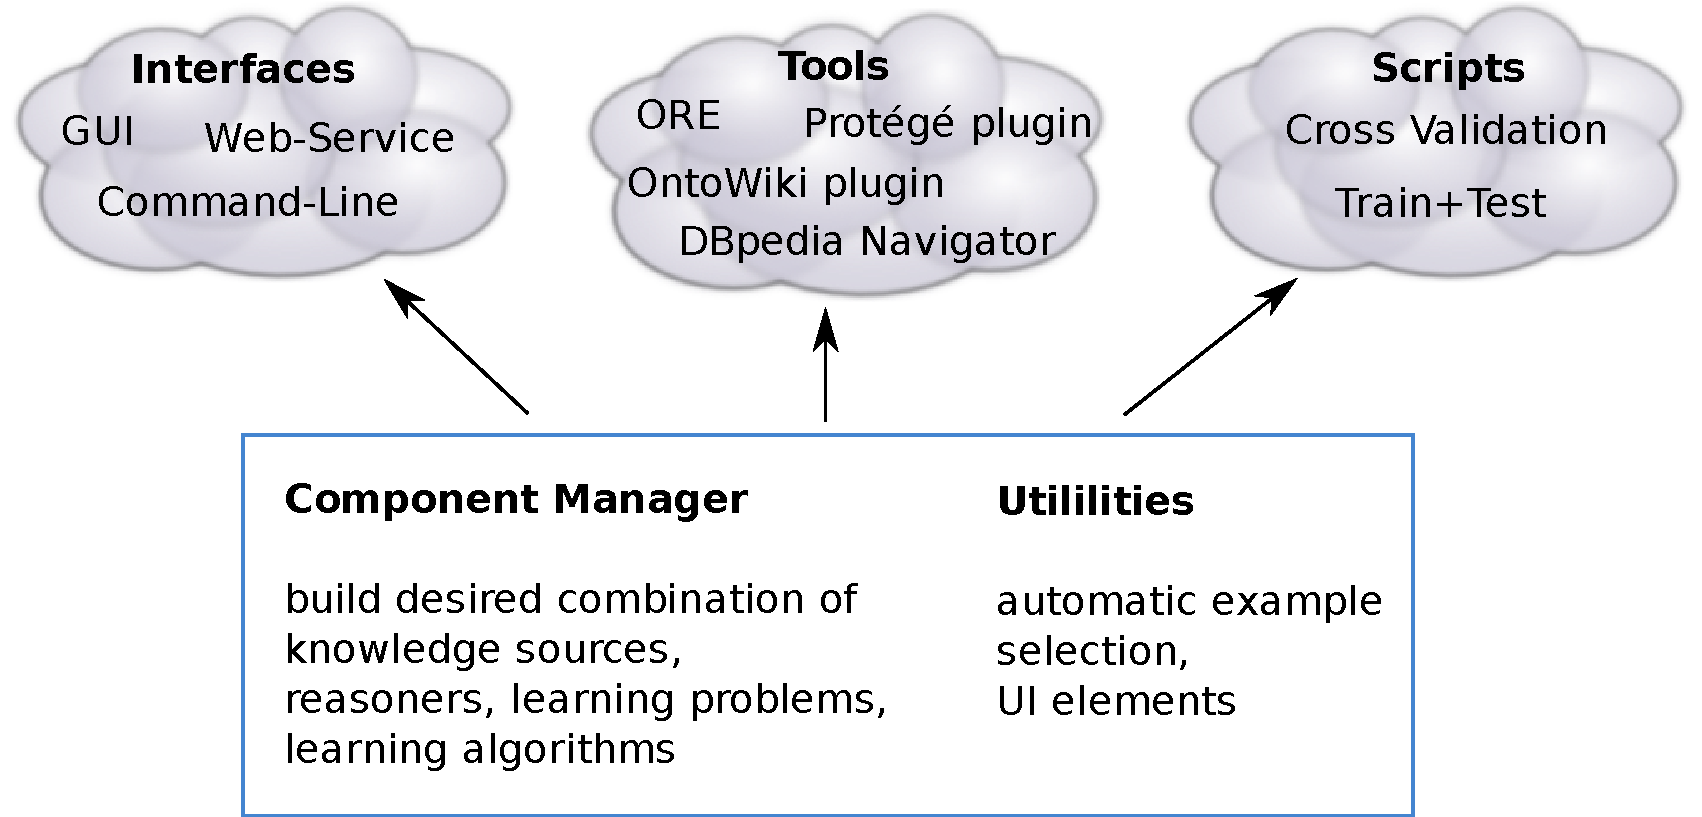
\includegraphics[width=\textwidth]{../../../../images/structure_print.pdf}
 \caption{Overall structure of the DL-Learner software.}
 \label{fig:structure}
\end{figure}

To be flexible in integrating new learning algorithms, new kinds of learning problems, new knowledge bases, and new reasoner implementations, DL-Learner uses a component based model. Adding a component can be done by implementing the appropriate Java interface and adding appropriate annotations (more on that in Section \ref{sec:developing}).

There are five common types of components (knowledge source, reasoning service, learning problem, learning algorithm, refinement operator). DL-Learner is not restricted to those types, i.e.~others can easily be added, but we limit ourselves to those five to make this manual easier to read. For each type, there are several implemented components and each component can have its own configuration options as illustrated in Figure \ref{fig:components}. Configuration options can be used to change parameters/settings of a component. In Section \ref{sec:components}, we describe the components in DL-Learner and their configuration options.

\begin{figure}[t]
  \centering
  %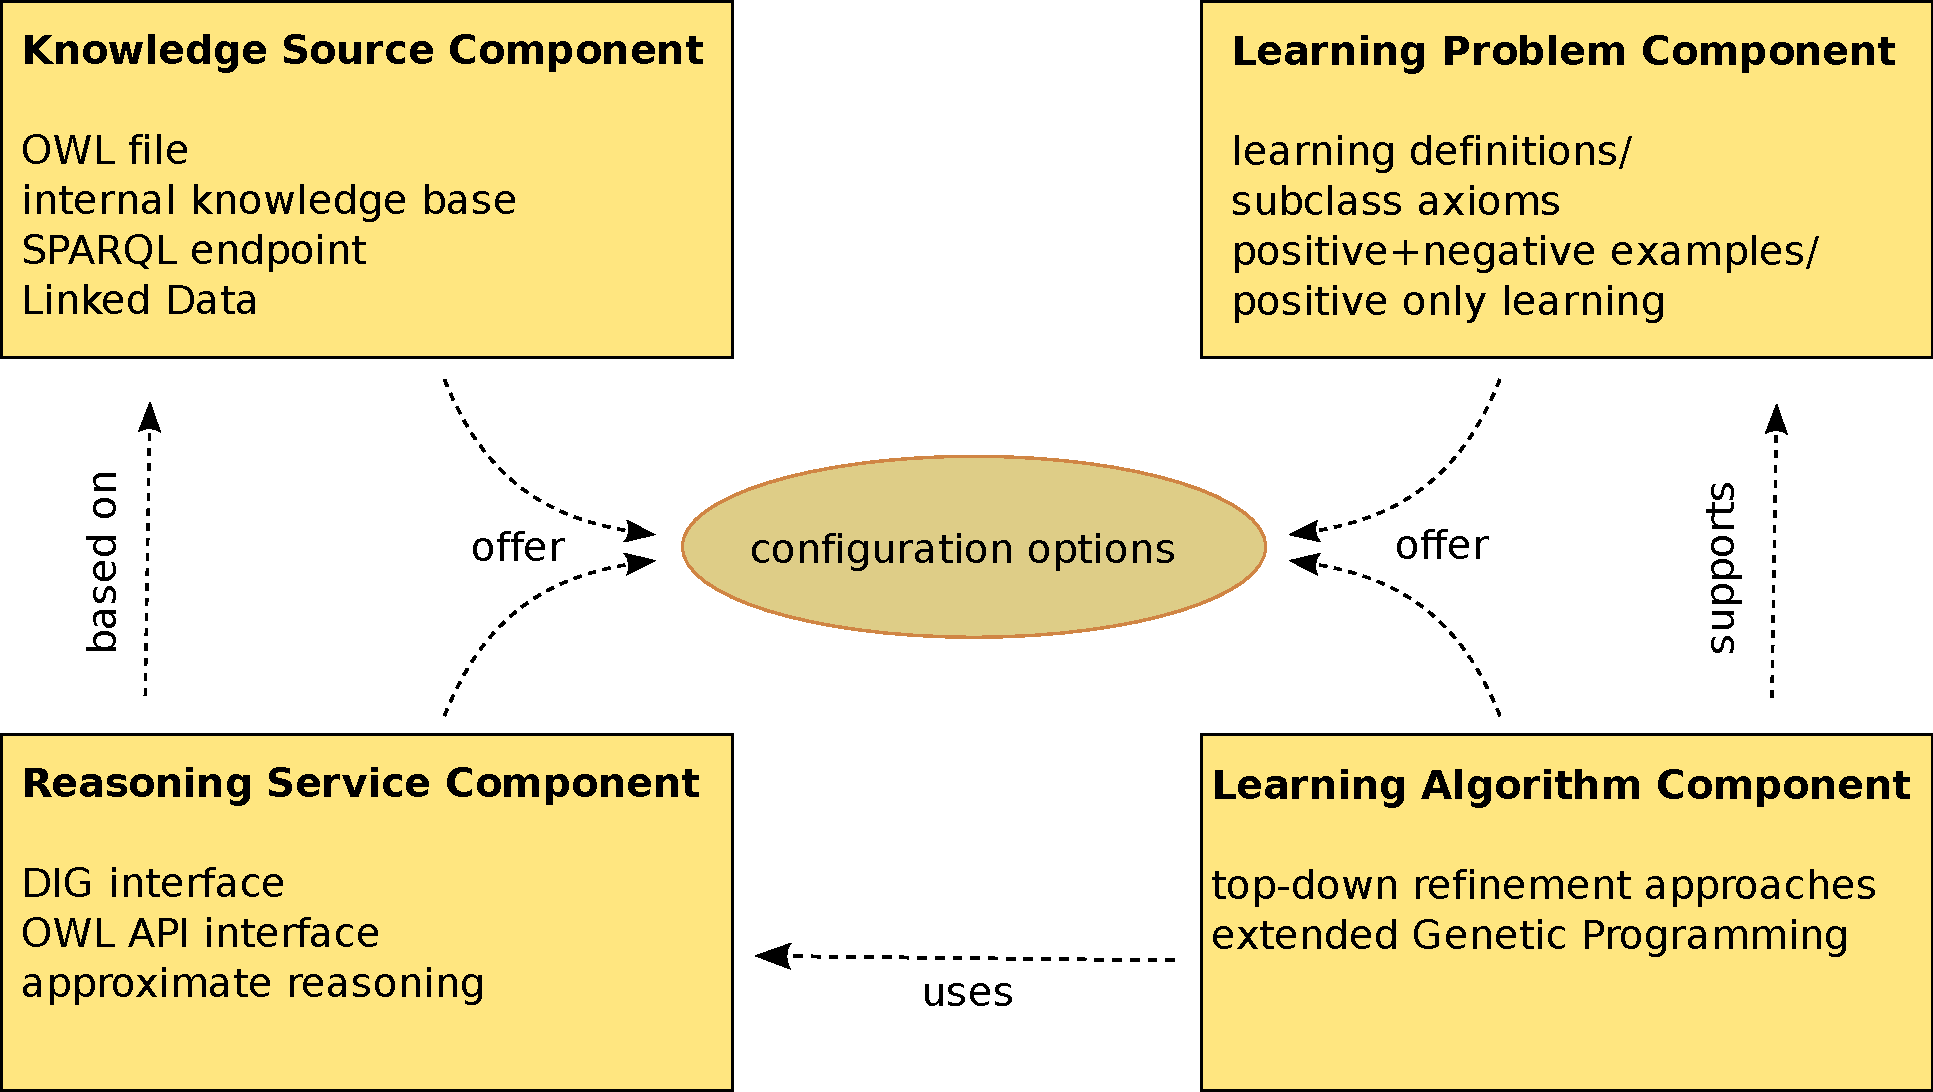
\includegraphics[width=\textwidth]{../../../../images/components_print.pdf}
  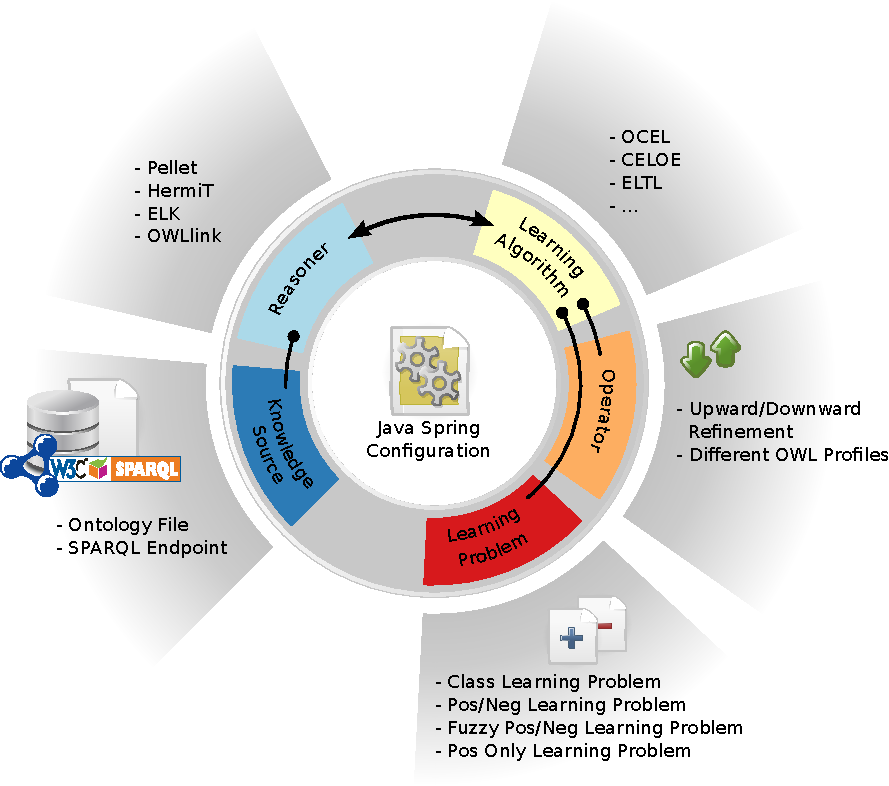
\includegraphics[width=.70\textwidth]{../../../../images/components.pdf}
  \caption{The architecture of DL-Learner is based on four component types, which can each have their own configuration options. DL-Learner uses a component manager to organise all components.}
  \label{fig:components}
\end{figure}

\section{DL-Learner Components}
\label{sec:components}

In this part, we describe concrete components currently implemented in DL-Learner. Each of the subsections contains a list of components according to the type specified in the subsection heading. Note that this does not constitute a full description, i.e.~we omit some components and many configuration options. The purpose of the manual is to obtain a general understanding of the implemented components. A full list, which is generated automatically from the source code, can be found in \verb|interfaces/doc/configOptions.html| including the default values for all options and their usage in conf files. The file is also available online at \url{http://htmlpreview.github.io/?https://github.com/AKSW/DL-Learner/blob/master/interfaces/doc/configOptions.html}.

\subsection{Knowledge Sources}
\label{sec:knowledgesources}

%Knowledge sources have a URI and can be included in conf files using \verb|import("$url");|, e.g.~\verb|import("ontology.owl")|. Depending on the file ending, DL-Learner will guess the correct type of knowledge source. If you want to overwrite this, you can use a second parameter with value \verb|OWL|, \verb|KB|, or \verb|SPARQL|, e.g.~\verb|import("ontology.owl","OWL")|.
The following contains some knowledge sources implemented in DL-Learner. To give an example, this is how a local OWL file can be declared as knowlege source in a conf file:
\begin{verbatim}
ks.type = "OWL File"
ks.fileName = "father.owl"
\end{verbatim}

\begin{description}
 \item[OWL File] DL-Learner supports OWL files in different formats, e.g. RDF/XML or N-Triples. If there is a standard OWL format, you want to use, but is not supported by DL-Learner please let us know. We use the OWL API for parsing, so all formats supported by it can be used\footnote{ for a list see \owlapi}.
 \item[KB File] KB files are an internal non-standardised knowledge representation format, which corresponds to description logic syntax except that the special symbols have been replaced by ASCII strings, e.g.~\verb|AND| instead of $\sqcap$. You can find several KB files in the examples folder. A description of the syntax is available online\footnote{\url{https://raw.githubusercontent.com/AKSW/DL-Learner/master/interfaces/doc/kbFileSyntax.txt}}. If in doubt, please use the standard OWL syntax formats.
%The \verb|doc/kbFileSyntax.txt| contains an EBNF description of the language.
 \item[SPARQL Endpoint] DL-Learner allows to use SPARQL endpoints as background knowledge source, which enables the incorporation of very large knowledge bases, e.g. DBpedia\cite{2008_dbpedia}, in DL-Learner. This works by using a set of start instances, which usually correspond to the examples in a learning problem, and then retrieving knowledge about these instances via SPARQL queries. The obtained knowledge base fragment can be converted to OWL and consumed by a reasoner later since it is now sufficiently small to be processed in reasonable time. Please see \cite{2009_ijswis} for details about the knowledge fragment extraction algorithm. Some options of the SPARQL component are:
\begin{itemize}
 \item instances: Set of individuals to use for starting the knowledge fragment extraction. Example use in conf file: \begin{verbatim}sparql.instances = {"http://dbpedia.org/resource/Matt_Stone",
 "http://dbpedia.org/resource/Sarah_Silverman"}\end{verbatim}
 \item recursionDepth: Maximum distance of an extracted individual from a start individual. This influences the size of the extracted fragment and depends on the maximum property depth you want the learned class expression to have. Example use in conf file: \verb|sparql.recursionDepth = 2|.
\item saveExtractedFragment: Specifies whether the extracted ontology is written to a file or not. If set to true, then the OWL file is written to the cache dir. Example usage: \verb|sparql.saveExtractedFragment = true|
\end{itemize}
 Many further options allow to modify the extracted fragment on the fly or fine-tune the extraction process.
The extraction can be started separately by running and modifying \verb|org.dllearner.test.SparqlExtractionTest|. The collected ontology will be saved in the DL-Learner directory.
\end{description}

\subsection{Reasoner Components}

Several reasoner components are implemented, which can be interfaces to concrete reasoner implementations. 
%To select a component in a conf file, use \verb|reasoner=$value;|, where  \verb|$value| is one of \verb|digReasoner|, \verb|closedWorldReasoner|, or \verb|owlAPIReasoner|, which are explained below.
Note that OWLlink reasoners can be attached via the OWL API interface.

\begin{description}
 \item[OWL API] The OWL API reasoner interface can be used in conjunction with the Pellet, FaCT++, HermiT and OWLlink reasoners. The only option allows to switch between them:
 \begin{itemize}
  \item reasonerType: Selects the desired reasoner. By default, Pellet is used. Usage: \verb|owlAPIReasoner.reasonerType = fact|. Pellet, FaCT++ and HermiT are already included in DL-Learner. Note that for FaCT++, you need to add -Djava.library.path=lib/fact/64bit (or 32bit) to the Java command. You can also use an external OWLlink reasoner by setting the reasoner type to \verb|owllink|. You can then use the option \verb|owlLinkURL| to specify the URL of the OWLlink reasoner (http://localhost:8080/ by default).
 \end{itemize}
 \item[SPARQL Reasoner] \todo{Simon}
 \item[Closed World Reasoner] Instance checks, i.e.~testing whether an individual is instance of a class, is the major reasoner task in many learning algorithms. This reasoner is a self-development of the DL-Learner project. It remedies some problems related to Machine Learning and the Open World Assumption in OWL and therefore is not correct w.r.t.~OWL semantics. (See \cite{cheng00} Section 4 for an explanation.) Furthermore, it provides an improved performance for instance checks by precomputing some inferences and keeping them in memory. The closed world reasoner is build on top of any other reasoner component in DL-Learner.
\end{description}

\subsection{Learning Problems}

In the introductory Sections \ref{sec:whatis} and \ref{sec:start}, we described a specific learning problem where positive and negative examples are given. In practice different variations of similar problems occur. 
%You can switch between the different problems using \verb|problem=$value;|, where \verb|$value| is one of \verb|posNegLPStandard|, \verb|posOnlyLP|, \verb|classLearning|. The default is \verb|posNegLPStandard|.

\begin{description}
 \item[Positive and Negative Examples] Let the name of the background ontology be $\mathcal{O}$. The goal in this learning problem is to find an OWL class expression $C$ such that all/many positive examples are instances of $C$ w.r.t.~$\mathcal{O}$ and none/few negative examples are instances of $C$ w.r.t.~$\mathcal{O}$. As explained previously, $C$ should be learned such that it generalises to unseen individuals and is readable. The important configuration options of this component are obviously the positive and negative examples, which you can specify via, e.g.~\texttt{\small posNegLPStandard.positiveExamples = \{...\}}.
 \item[Positive Examples] This learning problem is similar to the one before, but without negative examples. In this case, it is desirable to find a class expression which closely fits the positive examples while still generalising sufficiently well. For instance, you usually do not want to have \verb|owl:Thing| as a solution for this problem, but neither do you want to have an enumeration of all examples.
 \item[Class Learning] In class learning, you are given an existing class $A$ within your ontology $\mathcal{O}$ and want to describe it. It is similar to the previous problem in that you can use the instances of the class as positive examples. However, there are some differences, e.g.~you do not want to have $A$ itself as a proposed solution of the problem, and since this is an ontology engineering task, the focus on short and readable class expressions is stronger than for the two problems mentioned before. The learner can also take advantage of existing knowledge about the class to describe.
\end{description}

\subsection{Learning Algorithms}

The implemented algorithms vary from very simple (and usually inappropriate) algorithms to sophisticated ones.
Learning algorithms can make use of a refinement operator (see Sec.~\ref{sec:refinementoperators}) to traverse the search space.

\begin{description}
 \item[OWL Class Expression Learner (OCEL)]
 The general idea of the OCEL algorithm is to build a search tree based on a refinement operator and making use of a heuristic guiding the traversal of the search space.
 While the refinement operator defines how new candidate concepts may be derived from concepts already in the search tree, the heuristic can be configured to find \emph{`good'} candidates to look at (e.g. w.r.t. the concept length, its specificity and the number of covered examples).
 
 The OCEL algorithm supports double datatypes and hasValue restrictions (which again can be turned on or off as desired).
 It also includes explicit noise handling through the \verb|noisePercentage| option.
 More than 30 options can be set to control its behaviour.

 \item[Class Expression Learning for Ontology Engineering (CELOE)] Currently CELOE is the best class learning algorithm available within DL-Learner. It uses the same refinement operator as OCEL, but a completely different heuristics. Furthermore, it guarantees that the returned class expressions are minimal in the sense that one cannot remove parts of them without getting an inequivalent expression. Furthermore, it makes use of existing background knowledge in coverage checks. Statistical methods are used to improve the efficiency of the algorithm such that it scales to large knowledge bases. While it was originally designed for ontology engineering, it can also be used for other learning problems and might even be superior to the other algorithms in many cases (not well-tested yet). Note that many configuration options of OCEL were dropped for the sake of simplicity, but may be introduced if needed.
 \item[EL Tree Learner (ELTL)] This algorithm has EL as its target language, i.e. is specialized for this relatively simple language. There are two algorithms: \verb|el| learns EL concepts and \verb|disjunctiveEL| learns disjunctions of EL concepts.
 \item[Inductive Statistical Learning of Expressions (ISLE)]
 The ISLE approach \cite{Buehmann2014_short} is an extension of the ELTL algorithm, which can take standard knowledge sources (see Sec. \ref{sec:knowledgesources}) and textual evidence into account.
 An input corpus should contain textual descriptions of classes which support the generation on an ontology in an \emph{ontology learning} setting.
\end{description}

\subsection{Refinement Operators}
\label{sec:refinementoperators}

Refinement operators define a mapping from a given input concept description to a set of derived, or \emph{refined} concept descriptions.
In general there are to kinds of refinement operators: 1) \emph{upward refinement operators}, returning refined concept descriptions that are more general than the input concept description, and 2) \emph{downward refinement operators} returning concept descriptions that are more specific than the input concept description.
The specificity/generality here refers to the concept hierarchy in terms of subclass-of relations of concept descriptions.

Besides this, refinement operators differ in their expressiveness, i.e. the types of DL constructs they support.
As an example, the \texttt{rho} \emph{Rho (downward) refinement operator} can be configured to create refinements that contain cardinality restrictions, which is not supported by the \texttt{eldown} \emph{EL Downward refinement operator}.

A list of available refinement operators is given in the components and configuration settings document.

\section{Enrichment using DL-Learner}

Enrichment is usually a semi-automatic process, which adds information to an existing knowledge base.
Enrichment suggestions generated by an algorithm should be reviewed by a knowledge engineer who can then decide to accept or reject it.
Because of this, there is a need for serialising enrichment suggestions such that the generation of them is independent of the process of accepting or rejecting them.
Since all enrichment suggestions are OWL axioms, they could simply be written in an RDF or OWL file.
However, this might be insufficient, because we lose a lot of metadata this way, which could be relevant for the knowledge engineer. 
For this reason, DL-Learner uses an enrichment ontology, which is partially building on related efforts in~\cite{ontchange} and \url{http://vocab.org/changeset/schema.html}. 
Such an interchange format is also relevant, because the process of generating enrichments for all schema elements in very large knowledge bases will often take several hours to complete.
Furthermore, it may be desirable to include sufficient metadata to be able to reproduce algorithm runs for creating enrichment suggestions.
We briefly describe the main elements of the enrichment ontology.

\subsection*{Classes}

\begin{description}
  \item[Suggestion] Base class for enrichment suggestions.
  \begin{description}
    \item[AddSuggestion] Contains suggestions for adding axioms to an ontology.
    \item[RemoveSuggestion] Contains suggestions for removing axioms from an ontology.
  \end{description}
  \item[SuggestionSet] This class is used to group several suggestions with similar characteristics, e.g.~those generated by the same run of an algorithm.
  \item[Algorithm] The class containing all algorithms.
  \item[Creation] Contains all processes of creating a suggestion.
  \begin{description}
    \item[Manual] Manual enrichment suggestion processes, e.g.~a person suggesting a particular change to an ontology.
    \item[Automatic] Automatic and semi-automatic enrichment suggestions.
    \begin{description}
      \item[AlgorithmRun] Contains runs of a particular algorithm.
    \end{description}
  \end{description}
  \item[Parameter] Contains parameters of an algorithm.
  \item[Change] Actually performed changes in an ontology, e.g.~an accepted suggestion could become an instance of Change. This can be used to track which changes have already been performed as result of the enrichment process.
  \item[ChangeSet] A set of instances of Change.
\end{description}

\subsection*{Object Properties}

\begin{description}
  \item[hasSuggestion] Links a set of suggestions to its elements.
    \begin{description}
      \item[Domain:] SuggestionSet
      \item[Range:] Suggestion
    \end{description}
  \item[hasAxiom] Connects a suggestion to the axiom contained in it. Currently, this axiom is stored as Manchester OWL Syntax text string. 
  \begin{description}
      \item[Domain:] Suggestion
  \end{description}
  \item[hasParameter] Links to a parameter of an algorithm.
    \begin{description}
      \item[Domain:] AlgorithmRun
      \item[Range:] Parameter
    \end{description}
  \item[creator] Specifies who or what has created a set of enrichment suggestions.
    \begin{description}
      \item[Domain:] SuggestionSet
      \item[Range:] Creation
    \end{description}
  \item[usedAlgorithm] Specifies the used algorithm
    \begin{description}
      \item[Domain:] AlgorithmRun
      \item[Range:] Algorithm
    \end{description}
  \item[hasInput] Can be used specify input resources of an algorithm, for instance SPARQL endpoints.
    \begin{description}
      \item[Domain:] AlgorithmRun
    \end{description}
\end{description}

\subsection*{Data Properties}

\begin{description}
  \item[confidence] The confidence with which a Creator made a suggestion. The confidence is value between 0 and 1 with 0 indicating no confidence and 1 indicating absolute confidence.
    \begin{description}
      \item[Domain:] Suggestion
      \item[Range:] xsd:double
    \end{description}
  \item[explanation] A textual explanation why a suggestion was given. This could be a remark made by a person or a summary of statistical analysis results of an algorithm.
    \begin{description}
      \item[Domain:] Suggestion
    \end{description}
  \item[parameterName] The name of a parameter of an algorithm.
    \begin{description}
      \item[Domain:] Parameter
    \end{description}
  \item[parameterValue] The value of a parameter of an algorithm.
    \begin{description}
      \item[Domain:] Parameter
    \end{description}
  \item[timestamp] Timestamp of the start of automatic process.
    \begin{description}
      \item[Domain:] Automatic
    \end{description}
  \item[version] The version of the used algorithm.
    \begin{description}
      \item[Domain:] Algorithm
    \end{description}
\end{description}

To run the above enrichment algorithms on a SPARQL endpoint, you can use the provided enrichment script of DL-Learner.
It is a commandline interface, which you can start with ``./enrichment'' in Unix systems and ``enrichment.bat'' Windows systems.
Figure~\ref{fig:cli} shows the help screen, which is printed when running \verb|enrichment -?|.
We will briefly explain the options: 

\verb|-e| and \verb|-g| are used to specify the used endpoint and optionally a graph in this endpoint.

\verb|-r| is used to specify the resource (property or class), which should be enriched.
The system automatically determines whether this resource is a class, object property or data property and runs the corresponding algorithms. If this parameter is omitted, enrichment for the complete knowledge base is performed, i.e.~the system loops over all classes and properties in the SPARQL endpoint and generates enrichments.

The \verb|-f| switch can be used to control the format of the output.
By default, the suggestions are just printed to the console, but they can also be saved in a file in combination with the \verb|-o| option, e.g.~using the previously described enrichment ontology. 
This is useful for decoupling the enrichment suggestion generation process from the actual presentation of those suggestions to a knowledge engineer.

The \verb|-i| switch allows to turn inference on or off. If it is turned on, schema knowledge is loaded into a reasoner in the first step. Powerful reasoning capabilities may improve the quality of suggestions, in particular for those axioms, which rely on knowing the class hierarchy of the knowledge base, e.g.~domain and range axioms.

\verb|-t| allows to specify a threshold for enrichment suggestions, i.e.~suggestions with a lower score will be omitted. 

% \verb|-v| allows to turn on more verbose output on the command line.

\begin{figure}[tbh]
\begin{verbatim}
Option                        Description                            
------                        -----------                            
-?, -h, --help                Show help.                             
-e, --endpoint <URL>          SPARQL endpoint URL to be used.        
-f, --format                  Format of the generated output (plain, 
                                rdf/xml, turtle, n-triples).         
                                (default: plain)                     
-g, --graph [URI]             URI of default graph for queries on    
                                SPARQL endpoint.                     
-i, --inference [Boolean]     Specifies whether to use inference. If 
                                yes, the schema will be loaded into  
                                a reasoner and used for computing    
                                the scores. (default: true)          
-o, --output [File]           Specify a file where the output can be 
                                written.                             
-r, --resource [URI]          The resource for which enrichment      
                                axioms should be suggested.          
-t, --threshold [Double]      Confidence threshold for suggestions.  
                                Set it to a value between 0 and 1.   
                                (default: 0.7)                       

Additional explanations: The resource specified should be a class, 
object property or data property. DL-Learner will try to automatically 
detect its type. If no resource is specified, DL-Learner will generate 
enrichment suggestions for all detected classes and properties in the 
given endpoint and graph. This can take several hours.
\end{verbatim}
\caption{Depiction of the help screen of the enrichment script.}
\label{fig:cli}
\end{figure}

\section*{Examples}

Obtain enrichment suggestions for the \verb|currency| property in DBpedia:
\begin{verbatim}
-e http://dbpedia.org/sparql -g http://dbpedia.org 
-r http://dbpedia.org/ontology/currency
\end{verbatim}

Output those enrichments to a file \verb|results.txt|:
\begin{verbatim}
-e http://dbpedia.org/sparql -g http://dbpedia.org 
-r http://dbpedia.org/ontology/currency -o results.txt
\end{verbatim}

Write the enrichments in Turtle syntax in a file using the enrichment ontology:
\begin{verbatim}
-e http://dbpedia.org/sparql -g http://dbpedia.org 
-r http://dbpedia.org/ontology/currency -o results.ttl
-f turtle
\end{verbatim}

Do the same task with an increased threshold and without inference

\begin{verbatim}
-e http://dbpedia.org/sparql -g http://dbpedia.org 
-r http://dbpedia.org/ontology/currency -o results.ttl
-f turtle -t 0.9 -i false
\end{verbatim}

Generate all enrichments for DBpedia (will take several hours to complete):
\begin{verbatim}
-e http://dbpedia.org/sparql -g http://dbpedia.org 
\end{verbatim}


\section{DL-Learner Interfaces}

% \subsection{Command Line Interface}

%\todo{Description of Conf File Syntax; special cases: empty set of beans is denoted by ``-''; the name of a bean must not be ``true'' or ``false'' or start with a number; config options must not have the name ``type''; these conentions are introduced in order to be a able to provide a very compact syntax}

One interface you have already used in Section \ref{sec:start} is the command line. The main executable, which can be used for starting DL-Learner on the commandline is \verb|cli| which takes a conf file as argument. There are a lot of conf files available in the \verb|/examples| directory, which you can use a base for your own experiments.

%\begin{figure}
% \centering
% 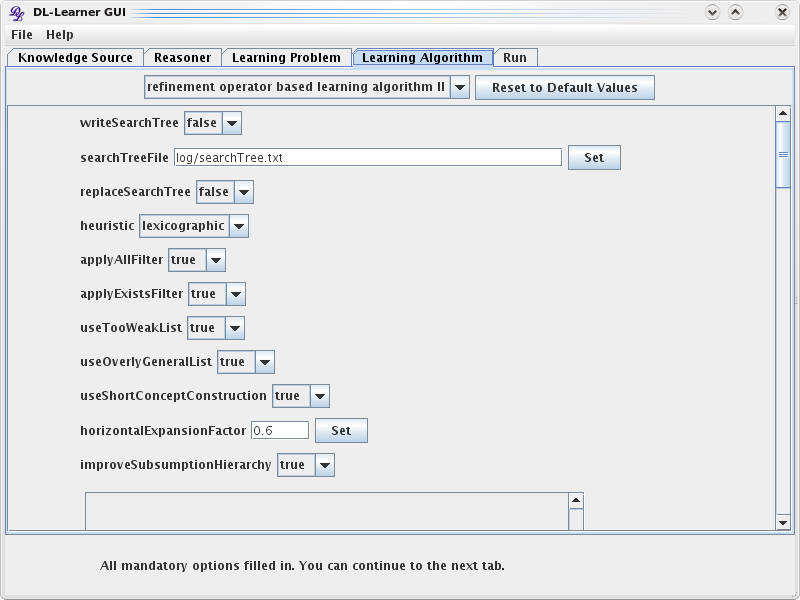
\includegraphics[width=.8\textwidth]{screenshots/gui_algorithm}
% \caption{GUI screenshot showing the learning algorithm tab. The UI allows you to set different options and then proceed to the next tab and execute the algorithm.}
% \label{fig:gui}
%\end{figure}

%DL-Learner had a graphical user interface and a web service. In 2011, DL-Learner was generalised to be able to solve general learning problems and arbitrarily combine components, which was necessary for learning SPARQL queries and fuzzy OWL class expressions. The commandline interface has been adapted for this purpose, but the graphical user interface and web service are currently under construction and will be re-introduced at a later stage.

% Web Service and GUI "under construction" at the moment

%Apart from the command line, there is also a prototypical graphical interface. You can use \verb|gui| (or \verb|gui.bat|) to start it. Optionally, a conf file can be passed as argument. The main GUI window has four tabs corresponding to the four different types of components and a run tab to execute the learning algorithm. Using the GUI, you can assemble the desired combination of components and options. The \verb|File| menu allows you to load a conf file or save the current configuration to a conf file. The GUI implementation is currently prototypical, so please report any bugs or feature requests you have (see Section \ref{sec:contact}). Since the GUI uses the component manager, it will automatically evolve when new components and options are added.

%A third interface through which DL-Learner can be accessed programmatically is a web service. You can execute \verb|ws| (or \verb|ws.bat|) to start the web service. It is based on the Java API for XML Web Services (JAX-WS), which is included in Java 6 or higher. Executing the command will start a web server on port 8181 of your local machine. The WSDL can be accessed via \url{http://localhost:8181/services?wsdl}. You can use a WSDL viewer to see the supported operations or view the JavaDoc of the corresponding Java file\footnote{viewable online at \wsjavadoc}. Some examples for calling the web service from PHP can be found in the DL-Learner subversion repository\footnote{in the directory src/php-examples/:\\ \wsphpexamples}.

Another means to access DL-Learner, in particular for ontology engineering, is to use the OntoWiki and Protégé plugins. The OntoWiki plugin is not officially released yet, but can be used in the SVN version of OntoWiki. The Protégé 5 plugin can be installed either by downloading it from the DL-Learner download page or directly within Protégé 4 by clicking on ``File'', ``Preferences'', ``Plugins'', ``Check for Downloads'' now and selecting the DL-Learner plugin. For more information and a screencast see the Protégé plugin wiki page \footnote{\wikiprotplugin}.

\section{Extending DL-Learner}
\label{sec:developing}

DL-Learner is open source and component based. If you want to develop a specific part or extension of a class expression learning algorithm for OWL, then you are invited to use DL-Learner as a base. This allows you to focus on the part you want to implement while being able to use DL-Learner as a library and access it through one of the interfaces. 

If you want to create a new component, then you first have to decide on the type of your component. To implement a concrete component, you can implement one of the following interfaces (list is incomplete):

\begin{itemize}
 \item org.dllearner.core.KnowledgeSource
 \item org.dllearner.core.ReasonerComponent
 \item org.dllearner.core.LearningProblem
 \item org.dllearner.core.LearningAlgorithm
\end{itemize}

%You then have to add your component to \verb|lib/components.ini| such that it is registered in the component manager when DL-Learner starts up. If you want to use configuration options in your component, you need to create a static method as follows:
That is sufficient for using your component programmatically in combination with existing DL-Learner components.
If your class name is \verb|org.example.TestAlgorithm|, then you can instantiate your class in a conf file via:
\begin{verbatim}
c.type = "org.example.TestAlgorithm"
\end{verbatim}

As you have probably seen by now in various conf files, DL-Learner allows to configure components. This is done via standard Java Beans. If you want to create a conf option \verb|testOption|, you just need to create a variable with getters and setters in your code:

\begin{verbatim}
public class TestAlgorithm implements LearningAlgorithm {

    private double testOption = 0.0;

    [...]

    public double getTestOption() {
        return testOption;
    }

    public void setTestOption(double testOption) {
        this.testOption = testOption;
    }

}
\end{verbatim}

That would be sufficient to include your components in conf files:
\begin{verbatim}
c.type = "org.example.TestAlgorithm"
c.testOption = 0.3
\end{verbatim}

In your code, you should have an empty default constructor and an \verb|init()| method (as required by the Component interface). The default constructor will be called first, followed by setter methods and then the \verb|init()| method. This is a standard Java Beans approach. In summary, you need to the following:
\begin{itemize}
	\item implement an appropriate DL-Learner interface for what you want to do
	\item add variables for all config options as well as getters and setters for them
	\item if you implement a constructor, please also add a default constructor with an empty set of arguments
\end{itemize}

By only requiring those few steps, we want to make adding further components to DL-Learner as lightweight as possible.
If you are familiar with the Spring framework\footnote{\url{http://www.springsource.org}}, then it is helpful to know that conf files are just an abbreviated syntax for Spring XML configurations. You can use all powerful features of Spring in your code, which we do not describe in full detail here. In fact, you can convert the conf files to Spring configuration files by adding those lines:

\begin{verbatim}
cli.type = "org.dllearner.cli.CLI"
cli.writeSpringConfiguration = true
\end{verbatim}

If you added this in \verb|test.conf|, then this generates a \verb|file.xml|, which is the Spring equivalent of conf file.

If you are a DL-Learner developer and want to properly document your component, you should do some further steps:
\begin{itemize}
	\item add an annotation for your class
	\item add annotations for all configuration options
\end{itemize}

An example of an annotated class could look as follows:

\begin{verbatim}
@ComponentAnn(name="Test Algorithm", shortName="ta", version=0.1, 
  description="My first experiment.")
public class TestAlgorithm implements LearningAlgorithm { ...

    @ConfigOption(defaultValue="0.0",
      description="The option allows to control xyz.")
    private double testOption = 0.0;

    [...]

    public double getTestOption() {
        return testOption;
    }

    public void setTestOption(double testOption) {
        this.testOption = testOption;
    }

}
\end{verbatim}

The \verb|@ComponentAnn| annotation allow to mark classes as DL-Learner components. Similarly, the \verb|@ConfigOption| annotations marks variables as configuration options. That should be those variables, which you want the user to be able to configure and play with. A benefit of adding the extra metadata provided by the annotations is that the component will appear in documentation pages\footnote{such as \url{http://htmlpreview.github.io/?https://github.com/AKSW/DL-Learner/blob/master/interfaces/doc/configOptions.html}}. In general, they provide users of your component with useful information.

\begin{comment}
You can then add your class to 

\begin{verbatim}
public static Collection<ConfigOption<?>> createConfigOptions() {
  List<ConfigOption<?>> options = new LinkedList<ConfigOption<?>>();
  options.add(new IntegerConfigOption("maxDepth", 
    "maximum depth of generated concepts/trees", 5));
  return options;
}
\end{verbatim}

This creates an option with name \verb|maxDepth|, the given description, and a default value of 5. To add further options, simply add more of them to the collection. If desired, running \verb|org.dllearner.scripts.ConfigJavaGenerator| generates a file for you in package \verb|org.dllearner.configurators| to access the options of your component programmatically. These configurator classes are particularly useful to build scripts or tools on top of DL-Learner components. An example for this can be found in \verb|org.dllearner.scripts.NewSample|.

Currently, the following configuration option types exist (new ones can be implemented if necessary):

\begin{itemize}
 \item boolean, e.g. \verb|useCache|
 \item string (a set of allowed strings can be specified), e.g. \verb|cacheDir|
 \item URL, e.g. \verb|reasonerURL|
 \item int (min and max value can be specified), e.g. \verb|maxDepth|
 \item double (min and max value can be specified), e.g. \verb|noisePercentage|
 \item set of strings, e.g. \verb|positiveExamples|
 \item list of string tuples, e.g. \verb|replaceObject|
\end{itemize}

Restricting to these option types this gives us the possibility to build very flexible user interfaces. Whenever, a new component or a new configuration option for a component is added, the current user interfaces (GUI, web service, commandline) will automatically support it without any or only minimal code changes.
\end{comment}

This quick introduction only serves as an entry point to get you started. For more detailed questions about how to extend DL-Learner, please drop us a message in the DL-Learner mailing list.

\section{General Information}
\label{sec:general}
\label{sec:contact}

\begin{itemize}
 \item Homepage: \url{http://dl-learner.org}
 \item GitHub project page: \url{https://github.com/AKSW/DL-Learner}
 \item Tracker (bugs, features): \url{https://github.com/AKSW/DL-Learner/issues}
 \item Mailing Lists: \url{http://sourceforge.net/p/dl-learner/mailman/}
 \item Contact: \href{mailto:jens.lehmann@cs.uni-bonn.de}{jens.lehmann@cs.uni-bonn.de} (please use the mailing list if possible)
 \item Latest Release: \url{https://github.com/AKSW/DL-Learner/releases/tag/v1.3}
\end{itemize}

\nocite{*}
\bibliographystyle{apalike}
\bibliography{manual.bib}

\end{document}

